% Chapter Template

\chapter{Data gathering and processing}
\label{Chapter2}
Data was sourced from several streams. The Icelandic Meteorological Office (IMO) provided measurements from weather stations all around Iceland. NWP data was downloaded from Copernicus Arctic Regional Reanalysis dataset (CARRA). A land elevation model was also provided by IMO.

\section{Automatic Weather Station Data}

IMO provided 10 minute measurements from \nStationsMin weather stations all around Iceland. The measurements that met the filtering criteria, started in \startDateVedur and ended in 2023. Of these \nStationsMin stations, \nVedurMin were from IMO and placed at 10 meters above ground, while the rest (\nVGMin) were from \href{https://www.vegagerdin.is/}{the Icelandic Road and Coastal Administration (IRCA)} and placed at 6-7 meters above ground\cite{vegagerdin_postur}. The location of these weather stations can be seen in Figure \ref{fig:aws_map}. The information that is provided by these Automatic Weather Stations (AWS) is presented in two different types of data files, hourly and 10 minute files. The hourly files are summations of the 10 minute files, with the exception that errors, such as nails, still in the 10 minute files should have been removed from the hourly documents. Nails, are sharp increases from the rest of the data and are unrealistic outliers that are considered measurement errors and are discarded. Each type of document contain the following information: the date and time, the station number (that can be converted to the coordinates using another data set), the average wind speed ($f$), the wind gust ($f_g$), the standard deviation of the wind gust, the direction of the wind ($d$) and the standard deviation for the wind direction. These measurement started at the end of the 20th century, when the first AWS stations was installed. More have been added in the following decades. This thesis does not look at the data as a time series, it tries to make predictions using only the information at a given point in time.

\begin{figure}
    \centering
    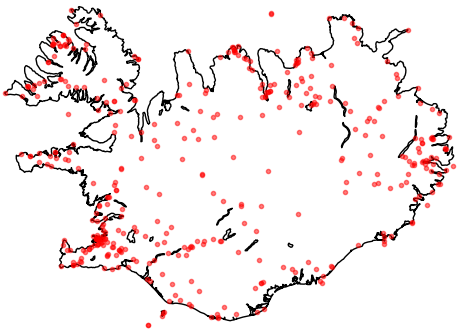
\includegraphics[scale = 1]{Figures/stationsOverIceland_2024-05-16_stripped_to_frame.png}
    \caption[Locations of automatic weather stations in Iceland]{Locations of all 412 stations that were looked at in this study. Most of these were from IMO but over a hundred were from IRCA. IMO AWS are placed at 10 meters above ground, while IRCA stations are placed at around 6-7 meters above ground.}
    \label{fig:aws_map}
\end{figure}

\section{CARRA Data}
The CARRA dataset goes back to September 1991 and is currently updated monthly, with a latency of 2-3 months\cite{carra_information}. The oldest IMO data point that fulfills given criteria is from \startDateVedur. This is covered by CARRA. The CARRA dataset is available for two regions, West and East. Each of these covers a vastly larger area than the area of interest. This leads to having to store a large amount of data. To get the data one has two options. Their web interface or using their API client. Using the API client is the only realistic option here, as there were thousands of requests made for different times. If using the API, it is possible to query a smaller area (such as a rectangular area around Iceland) given a set of coordinates.

The requests to the API are made at each available CARRA hour ([00, 03, 06, 09, 12, 15, 18, 21]) for each available observation. Only these hours can be used as the CARRA predicted output is represents the wind speed at those given hours and would thus not encapsulate well the extreme values in between these times. Using these datapoints, interpolation was used to get an estimation for the point of the given weather station. The CARRA data contains several types of layers. These are single levels, model levels, height levels, pressure levels. The data for this thesis was downloaded from height levels. That is, data was requested at heights of 15, 250 and 500 meters above ground. For each point 4 parameters were requested, wind speed, wind direction, pressure and temperature. Each of these features needed to be interpolated to create data for model to be trained on.

\section{Elevation data}
IMO provided a TIFF file containing the elevation of Iceland on a 20 meter by 20 meter grid. This file encompasses Iceland and is around 685 MB. The Python package Rasterio allowed for quick lookup with it's index and the affine transform. Using this package it is possible to quickly look up elevation given coordinates using matrix calculations. This package allowed for lookup by coordinates and by positioning inside the grid encompassing Iceland. It also allows for index lookup using coordinates. Using index lookup, neighboring points can be looked up and used to bridge the elevation for exact posisiton of given point.

\label{Chapter3} 
\section{Combining data sources}

This project used three main data sources, which need to be queried, filtered and combined to prepare the data for use in the models. When working with hundred of thousands of rows, the efficiency of the code is very important. Iterating through those rows might be necessary at times but will increase the time exponentially as compared to using vectorizing methods were possible. The three data sources were all in a different format. Measurement data from IMO was in text files, elevation data was in GeoTiff and reanalysis data from CARRA was in a GRIB format. To use the data to train, these three data sources needed to be combined into one file. This was done based on the measurement data from the IMO. A limit was set on the average wind speed and it was used to select measurement points. Along with the average wind speed having to be above a certain limit, to ensure that the same weather for the same location is not duplicated. The data from IMO was supplied for 10 minute increments, while CARRA data is in 3 hour intervals. This means that to use the CARRA data to predict the measured values from IMO, temporal interpolation would need to be done. Along with the temporal interpolation, note that the CARRA data is given in a rectangular grid where the distance between each point is around 2.5 km while the the information from the IMO is given at specific locations. The elevation information was given by a 20 by 20 rectangular grid that covers Iceland. When combining these data sources an interpolation method needs to be decided upon. Here linear interpolation was applied, both temporally and spatially. As the measurement points chosen were not outliers, that is the strongest average wind speed in a given range, interpolating in time does not work well. This necessitates using only measurements that are exactly at three hour intervals (00, 03, 06, 09, 12, 15, 18, 21 hours) at interpolating only in space. The choice of interpolation method, although potentially impactful on the results, was not specifically addressed in this study.

\begin{figure}[h]
    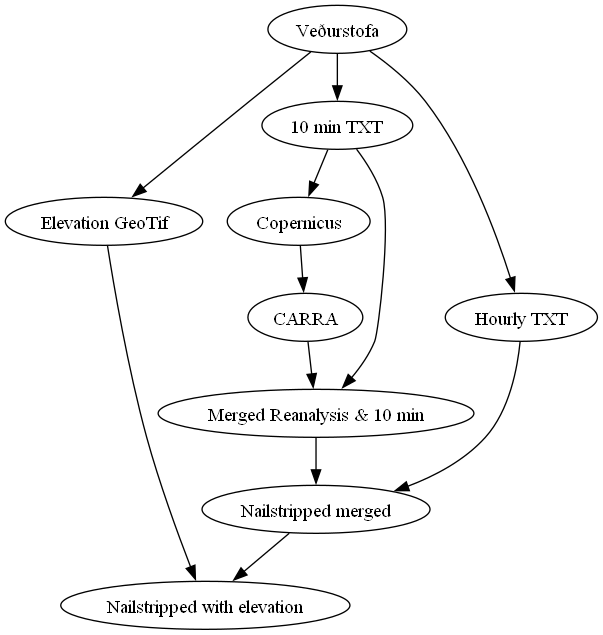
\includegraphics[scale = 0.5]{Figures/data-preprocessing-flow-chart.png}
    \caption{A flow chart showing how data sources were combined}
    \label{fig:data_preprocessing_flow_chart}
\end{figure}

The procedure of combining these sources was as follows and can be seen in Figure \ref{fig:data_preprocessing_flow_chart}. The measured data from the AWS is filtered by using a limit on the average wind speed. The gust factor generally drops with increased wind speed (although not always dependent on factors such as the landscape \cite{GNP_vidtal}). Even so being able to predict the gust factor is more important for higher average wind speed due to higher wind gusts. After this stripped dataset over every AWS has been created it is used to query the CARRA data by using their API. The CARRA API needs to be queried for given hours, days, months, years and a given area. That is, if queried for a given hour, it returns that hour for every day that is queried. Similarly if queried for a given day, it returns that day for every month. In light of these restraints, it was decided to query month by month. Querying only the days needed but every hour of the day (UTC 00, 03, 06, 09, 12, 15, 18 and 21). After querying and downloading the data for the height levels and variables requested, points of interest are interpolated and values stored in a pandas dataframe. After this the downloaded data is discarded and the next month is queried. This drastically decreases the amount of data that needs to be stored as compared to downloading the entire area and keeping all the data points (a reduction from several terabytes to less than a gigabyte).

Once CARRA data has been merged with AWS data, using station and time columns, then this combined file needs to checked for nails. This is done by using the hourly data (which is supposedly error free). As the data has been filtered in for the highest average wind speed in a 48 hour interval, the hourly data can be used to find nails. The hourly data is combined with the merged AWS and 10 min data. Then filtering is applied on the average wind. If the average wind speed for the 10 minute data is higher than the hourly the rows are dropped. Most stations have nails in less that 10\% measurements. The stations that have higher than 10\% error are ignored.

The elevation data comes in a GeoTIFF file that covers Iceland. It is a rectangular grid of resolution 20 meters. For every point of interest (every weather station), the elevation of that given point along with other points surrounding the weather station is retrieved. For each point retrieved interpolation needs to be done. This is done in a similar manner to the interpolation of the CARRA data. The four points bounding the point of interest were used to linearly interpolate the value of the point of interest. This information is included in the training data as the landscape is known to influence both the average wind and the gustiness \cite{GNP_vidtal}.

The error in reanalysis wind speed and measured wind speed can be significant. The absolute error increases as the measured wind speed increases, while the percentage wind speed decreases. A grouping of these errors by wind speed can be seen in Table \ref{table:measuredVSReanalysis_wind_speed}


\begin{table}[h]
    \caption[Comparison of measured and reanalysis wind speed]{Comparison of measured and reanalysis wind speed using mean absolute error (MAE) and mean absolute percentage error (MAPE). Note that for the computation of MAPE for ranges that otherwise include 0, 0 values have been excluded so as to prevent division by zero and exploding values. The comparisons are done using measured wind speed (at 10 meters above ground for IMO and 6-7 meters above ground for IRCA) and reanalysis wind speed at 15 meters above ground.}
    \label{table:measuredVSReanalysis_wind_speed}
    \centering
    \begin{tabular}{ccc}%c}
        \toprule
        f & n & MAE \\%& MAPE \\
        \midrule
        $[0;5[$ & 6.2e6 & 2.1 \\%& 1.6\\
        $[5;10[$ & 4.2e6 & 2.2 \\%& 0.3\\
        $[10;15[$ & 1.5e6 & 2.5 \\%& 0.2\\
        $[15;20[$ & 3.9e5 & 3.0 \\%& 0.2\\
        $[20;25[$ & 8.4e4 & 4.0 \\%& 0.2\\
        $[25;\infty[$ & 2.0e4 & 6.6 \\%& 0.2\\
        $[0;\infty[$ & 1.2e7 & 2.2 \\%& 1.0\\
        \bottomrule
    \end{tabular}
\end{table}

Another thing to look at is the distribution of error by station, both in terms of their coordinates and number of measurements. Looking at Figure \ref{fig:station_mae_distribution}, this distribution can be seen.

\begin{figure}
    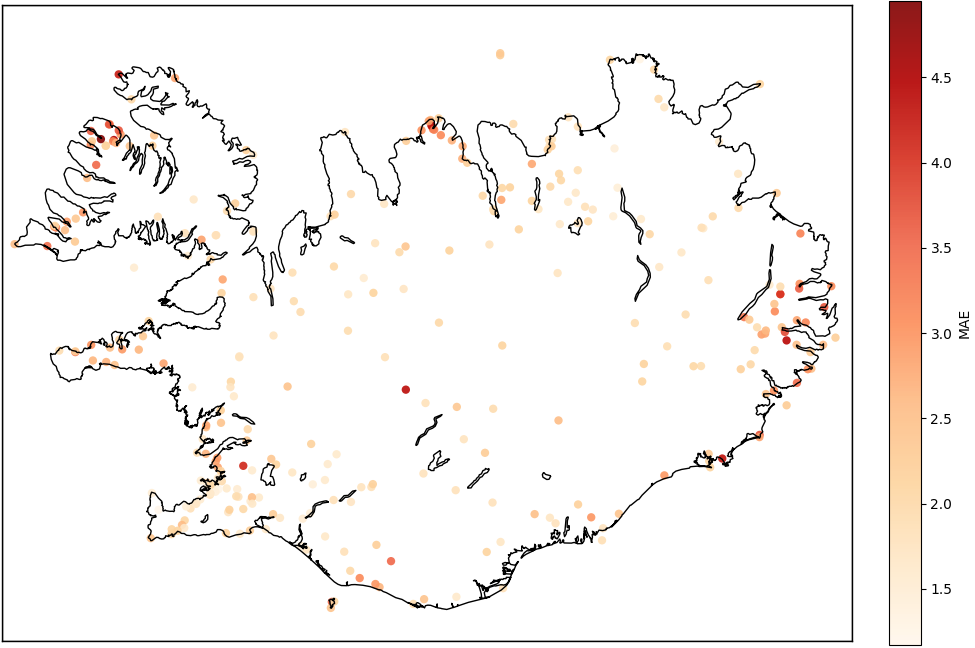
\includegraphics[scale=0.6]{Figures/MAEoverIceland.png}
    \caption[Distribution of mean absolute errors by station]{The distribution of mean absolute errors by station. Using mean absolute error instead of mean absolute percentage error allows for all points to be used. Mean absolute percentage error can only be used if 0 values are ignored.}
    \label{fig:station_mae_distribution}
\end{figure}

Table \ref{table:station_mae_distribution} shows the 5 best and worst stations in terms of MAE.

\begin{table}[h]
    \caption[Mean absolute difference of measured wind speed and reanalysis wind speed at select stations]{Mean absolute error for reanalysis wind speed as compared to measured wind speed, for the five stations with the highest difference and the five stations with the lowest difference.}
    \label{table:station_mae_distribution}
    \resizebox{\textwidth}{!}{
    \centering
    \begin{tabular}{cccc}
        \toprule
        Station & Number of measurements & MAE & Location \\
        \midrule
        1470 & 6.8e3 & 1.17 & Reykjavík Háahlíð \\
        1350 & 5.2e4 & 1.18 & Keflavíkurflugvöllur \\
        1482 & 1.4e4 & 1.23 & Reykjavík Víðidalur \\
        4921 & 1.3e4 & 1.29 & Rif á Melrakkasléttu \\
        1477 & 5.6e4 & 1.29 & Reykjavíkurflugvöllur\\ \hdashline[0.5pt/1pt]
        35553 & 4.0e3 & 4.30 & Almannaskarð - göng\\
        6745 & 1.5e4 & 4.36 & Kerlingarfjöll - Ásgarðsfjall\\
        35978 & 7.9e3 & 4.40 & Fáskrúðsfjarðargöng suður\\
        2640 & 1.6e3 & 4.51 & Seljalandsdalur\\
        32635 & 3.2e4 & 4.95 & Botn í Súgandafirði\\
        \bottomrule
    \end{tabular}
    }
\end{table}

If the 0 m/s is excluded from the measurement data, then the error distribution using MAPE can be plotted. This plot can be seen in Figure \ref{fig:station_mape_distribution}

\section{Data Structure}

Once data has been retrieved for all three sources and processed, including interpolating values, it needs to be made ready to use by the model, for both training, validation and test. The starting point is a dataframe that contains measured information from AWS. This includes the average wind, the wind gust, wind direction along with the station number and coordinates. When selecting the CARRA data certain height levels are chosen. These present as separate lines in the CARRA dataframe. Information for one observation is represented in as many lines as height levels requested in the reanalysis data. These rows need to be combined on the position (the weather station). When this is done it is possible to combine the AWS IMO data and CARRA reanalysis data on the location and time columns. The last data source is the elevation. A circle sector upwind is looked at. In any case the points, that represent these sections, were selected as shown in Code Listing \ref{code:sectorElevation}. A range of angles are defined based on the wind direction $d$ at some distance from the given point. This means that the resultant points (equal in number to the length of angleRange by k) from arcs at several distances from the given weather station.

\begin{lstlisting}[style = Python, caption = {Sector elevation points generated}, label = code:sectorElevation]
angles = [(angle + (90 - d)) * pi/180 for angle in angleRange]
length_rng = [(exp(i * log(n + 1)/ k) - 1) * 1000 
                for i in range(1, k + 1)]
points = np.array([[(X + l * cos(angle), Y + l * sin(angle))
                    for angle in angles] for l in length_rng])   
\end{lstlisting}

The result is a dataframe that has measured data from AWS, which gives us our target, reanalysis data from CARRA, which gives us weather variables to train on, and finally elevation points in the landscape to include in our training data. An example of what the data looks like can be seen in Table \ref{table:trainDataExample}.

\begin{table}[h]
    \caption[An example of data structure used to train model]{An example of data structure used to train model. Data points include the derived variables Ri and N, the elevation of the station, direction of wind and relative direction of the wind (twd, that is the direction of the wind relative to center of Iceland), along with some combination of wind speed, pressure and temperature at the different height levels. Finally there are the elevation points around a given station, where the elevation is relative to the station.}
    \label{table:trainDataExample}
    \resizebox{\textwidth}{!}{
    \centering
    \begin{tabular}{cccccccccc}
        \toprule
        Ri & $N^2$ & station elevation & twd & $ws_{15}$ & $wd_{15}$ & $t_{15}$ & $p_{15}$ & $elevation_0$ & \dots\\
        \midrule 
        -1.18e+00 &  2.67e+04 & 100 & 1.5 & 10 & 5 & 0 & 100 & 2 & \dots\\
        \bottomrule
    \end{tabular}
    }
\end{table}

Looking at Table \ref{table:trainDataExample} note that the first two columns represent two variables that describe the stability of the air. These are the Richardson number ($Ri$)\cite{richardson_number_skybrary} and Brunt–Väisälä frequency\cite{brunt_vaisala_freq_eumtrain} ($N$), and are calculated using Equations (\ref{eqn:Ri}) and (\ref{eqn:N})\cite{mean_gust_HA_HO}. These values are calculated using reanalysis data at two different height levels. Thus $Ri$ refers to the Richardson number calculated between height levels 15m and 500m. Exactly the same notation is used with the Brunt–Väisälä frequency, except the square is used.

\begin{equation}
    \label{eqn:Ri}
    Ri = \frac{g \cdot dT \cdot dz}{T_{\textrm ave} \cdot dU^2} \unit{[]}
\end{equation}

\begin{equation}
    \label{eqn:N}
    N = \sqrt{\frac{g \cdot dT }{T_{\textrm ave} \cdot dz}} \unit{[Hz]}
\end{equation}

Here, $g$ is the acceleration due to gravity, $dT$ is the temperature difference between the two height levels, $dz$ is the elevation difference, $T_{\textrm ave}$ is the average temperature (that is the average of the two temperatures in the height levels) and $dU$ is the wind speed difference between the two height levels. Both of these numbers provide some insight about the stability of the air. A lower value for the Richardson number indicates a higher turbulence. A typical range of values could be between 0.1 and 10, with values below 1 indicating significant turbulence\cite{richardson_number_skybrary}. When the square of the Brunt-Väisälä frequency is negative, then the air is unstable (an air parcel will move away from its original position)\cite{brunt_vaisala_freq_eumtrain}. These are derived factors from the reanalysis data and as such there shouldn't be a significant information gain using $Ri$ and $N$ as opposed to having the raw data. However, including these factors instead of every reanalysis variable requested might speed up training as well as making the model more easily explainable with the use of Shapley values or other tools for explainability. Using Shapley a feature importance value is attributed to a given feature by creating all possible permutations of any possible length (up to number of features) and seeing how the predictions are skewed when the given parameter is included or excluded. This needs to be done for all parameters. The time complexity of this is very high ($2^n$ coalitions)\cite{shapley_information}. Most implementations use some approximations, which still can take a considerable amount of time for models with a high parameter count and many examples. The Richardson number includes the difference in wind speeds in the denominator. In certain cases, where the difference in wind speed between two levels is very, can blow up to infinity. This can cause problems and distort the predicitons.

\section{Data distribution}

The CARRA data is reanalysis and as such might have a bias or some systemic distortion when compared to the measured data. The distribution of the observed and reanalysis wind speed can be seen in Figure \ref{fig:obs_carra_wind_speeds}. Looking at the figure, the reanalysis wind tends to be higher even though the distribution is similar. 

\begin{figure}[ht]
    \centering
    % First subfigure (top)
    \begin{subfigure}[b]{0.8\textwidth}
        \centering
        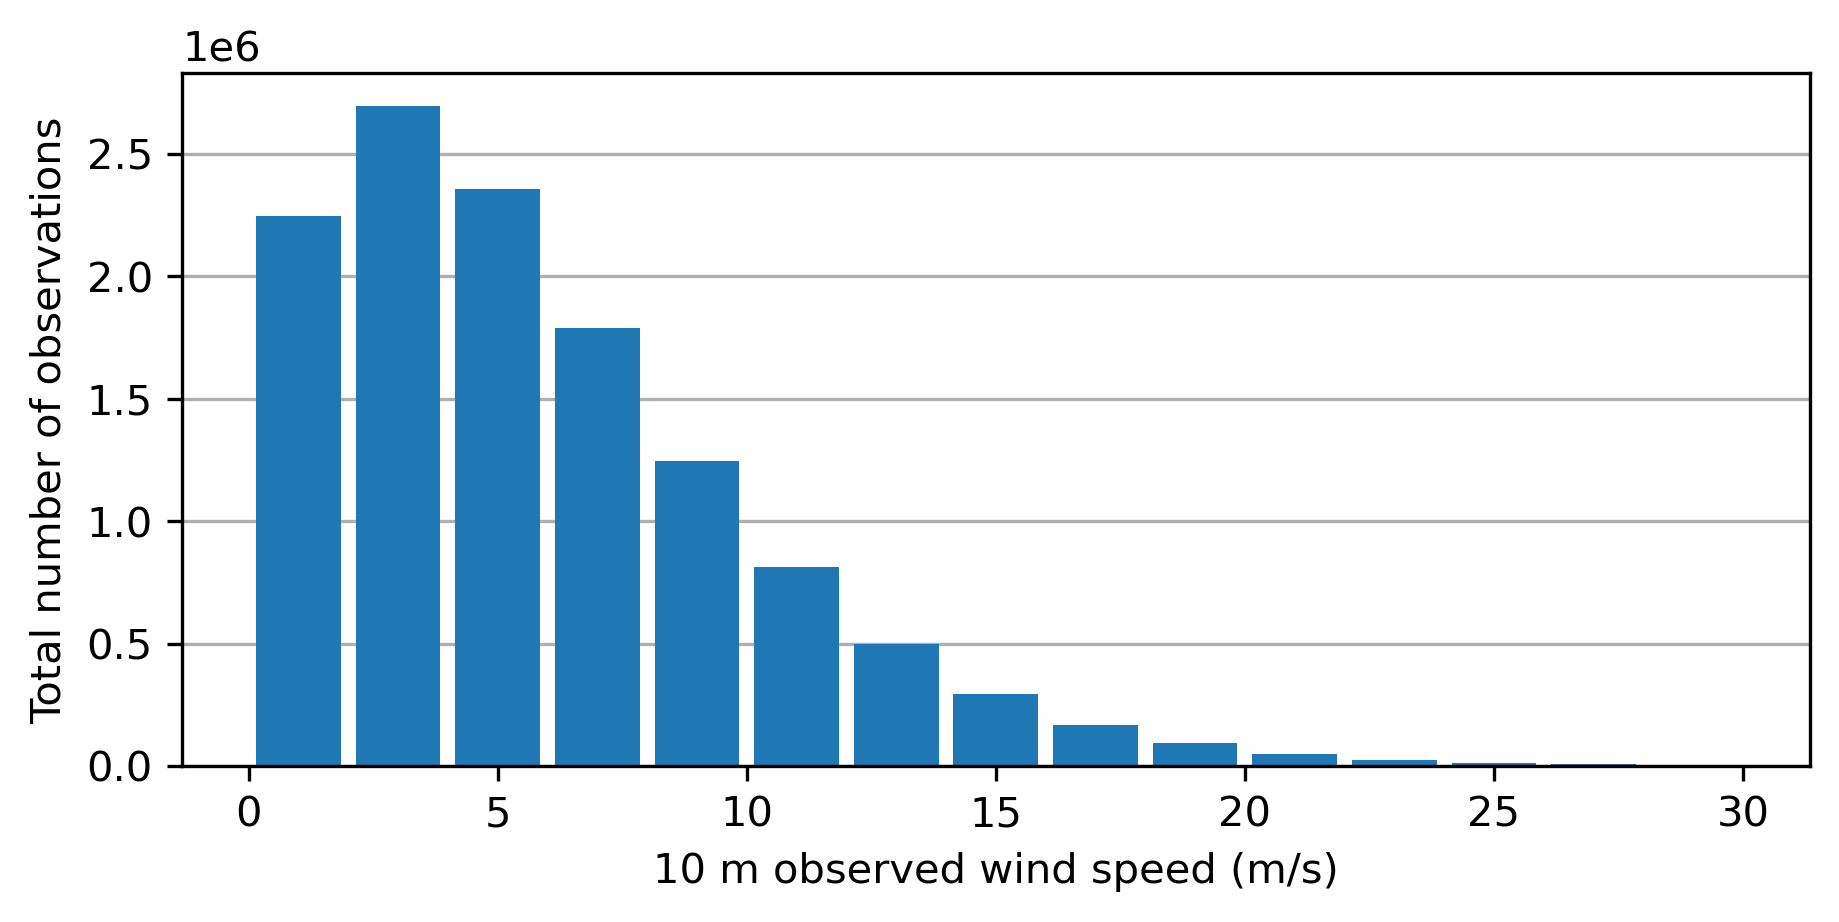
\includegraphics[width=\textwidth]{Figures/obs_wind_speeds.png}
        \caption[Histogram of observed wind speeds]{A histogram distribution of observed wind speeds provided by IMO and IRCA for all used weather stations.}
        \label{fig:obs_wind_speeds}
    \end{subfigure}
    
    \vspace{0.5cm} % Space between the two images

    % Second subfigure (bottom)
    \begin{subfigure}[b]{0.8\textwidth}
        \centering
        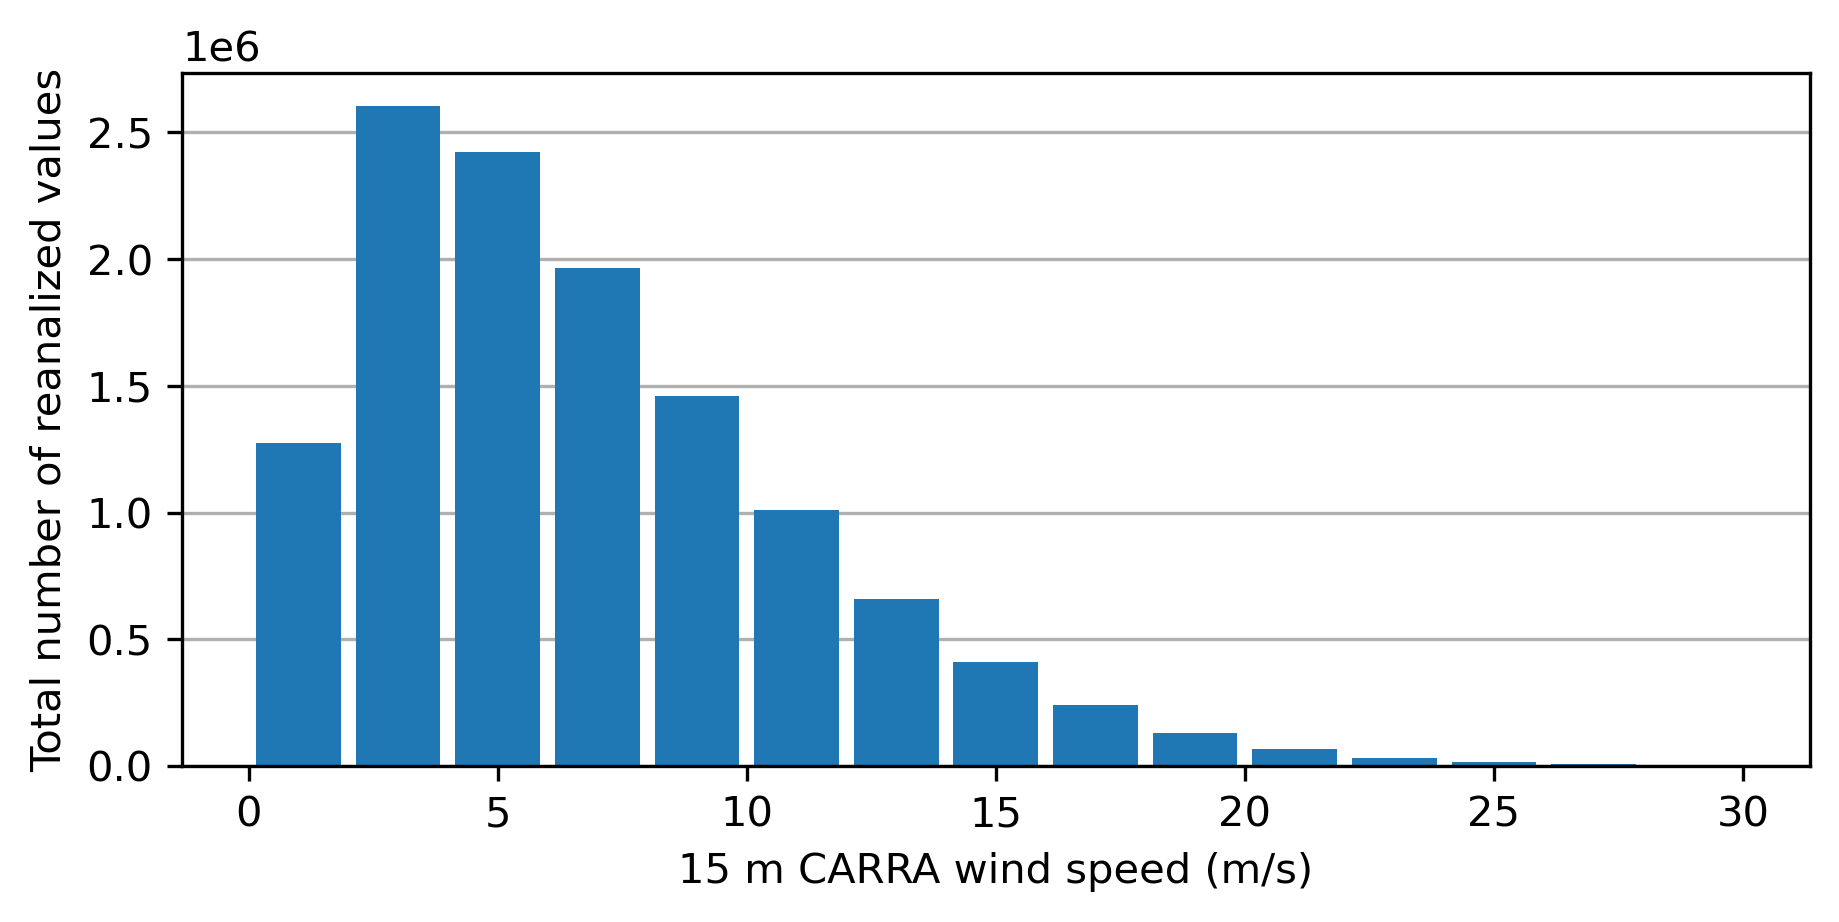
\includegraphics[width=\textwidth]{Figures/carra_wind_speeds.png}
        \caption[Distribution of interpolated CARRA wind speeds at weather stations]{Distribution of interpolated CARRA reanalysis values at weather stations. The reanalysis data is only available at 3 hour intervals and 2.5km grid. These values are interpolated from data given by CARRA at the weather stations.}
        \label{fig:carra_wind_speeds}
    \end{subfigure}

    \caption[Distribution of CARRA and observed wind speeds]{Distribution of CARRA reanalysis wind speed and observed wind speed at weather stations provided by}
    \label{fig:obs_carra_wind_speeds}
\end{figure}

\begin{figure}[ht]
    \centering
    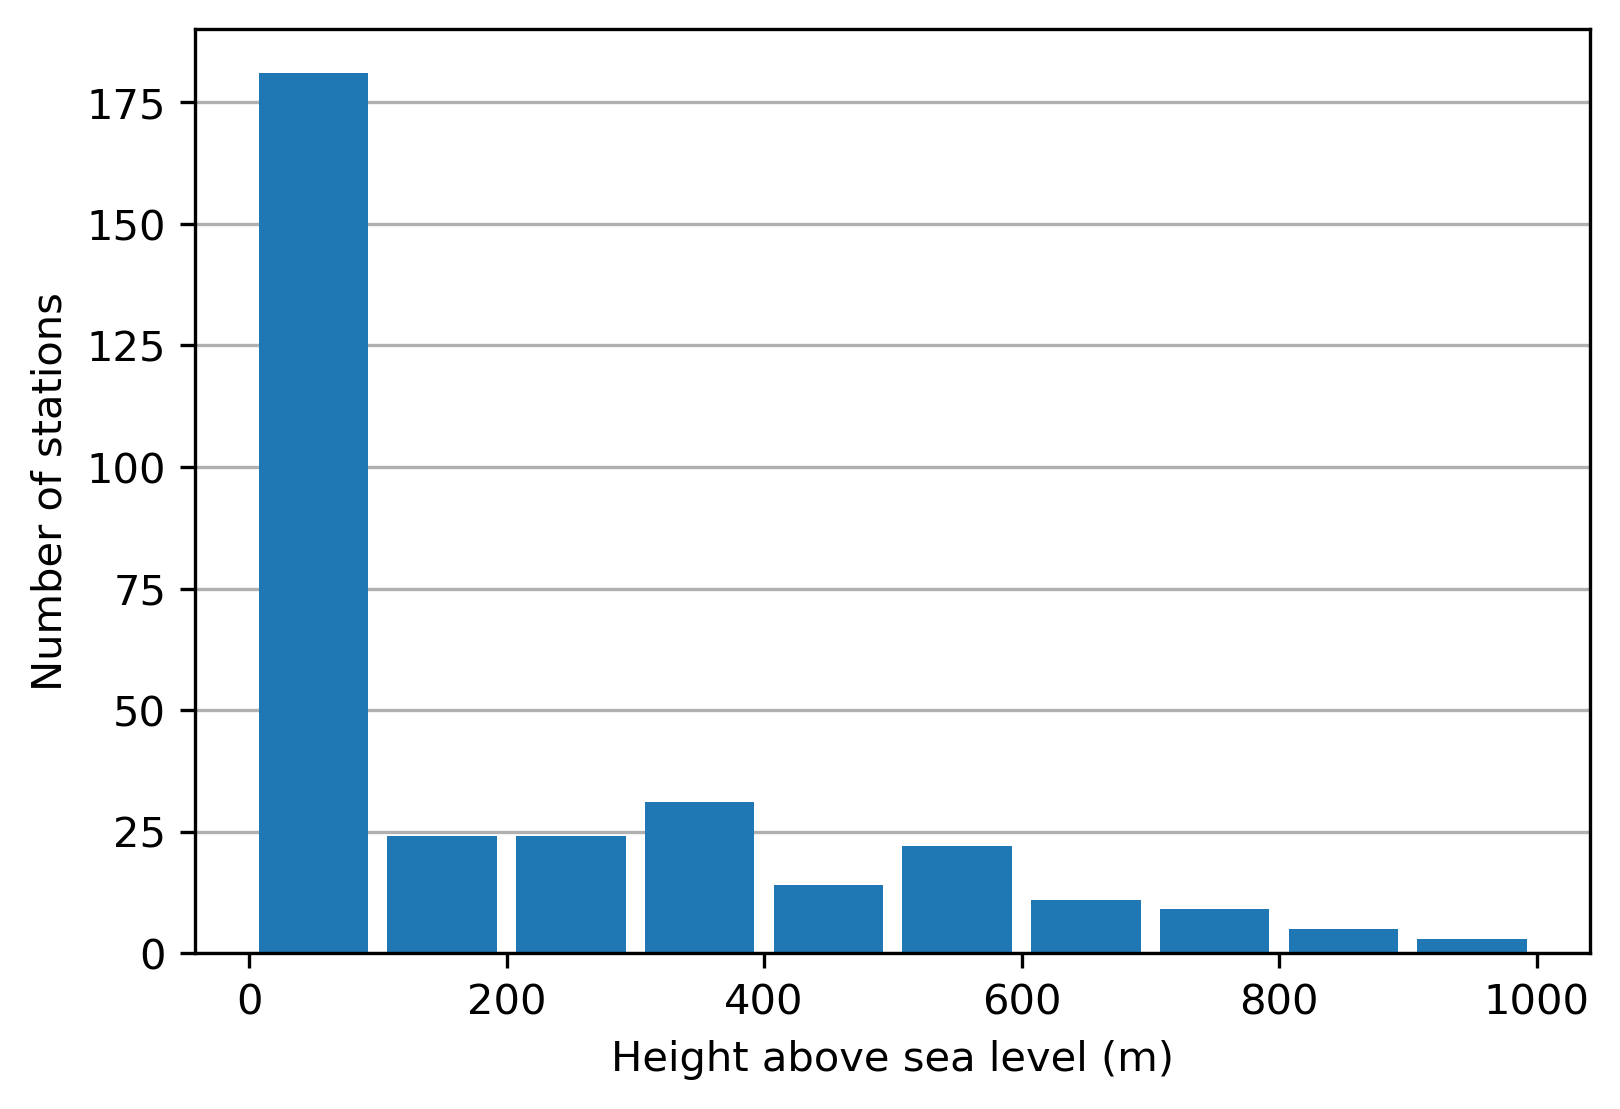
\includegraphics[width=0.8\textwidth]{Figures/station_heights.png}
    \caption[Distribution of weather station heights above see level]{Distribution of ...}
    \label{fig:station_heights}
\end{figure}